\documentclass[9pt,aspectratio=1610]{beamer}

\usepackage{color,fancybox,alltt,graphicx}

\usepackage{pgf,pgfarrows,pgfnodes,pgfautomata,pgfheaps,pgfshade}

\usepackage[latin1]{inputenc}
\usepackage{colortbl}
\usepackage[english]{babel}
\usepackage{multimedia}
\usepackage{amssymb,amsmath}
\usepackage{ragged2e}
\usepackage{animate}
\usepackage{listings}

\newif\ifpdf
\ifx\pdfoutput\undefined
\pdffalse % we are not running PDFLaTeX
\else
\pdfoutput=1 % we are running PDFLaTeX
\pdftrue
\fi

\mode<article>{ \usepackage{fullpage}  \usepackage{pgf}  \usepackage{hyperref} }


\mode<presentation>{
  \usetheme{XAFS}
  \setbeamercovered{transparent}
}

\usepackage{amsmath}
\usepackage{tikz}

\usepackage[customcolors,shade]{hf-tikz}

\usetikzlibrary{calc}

% put color to \boxed math command
\newcommand*{\cmboxcolor}{orange}
\makeatletter
\newcommand{\cmbox}[1]{\textcolor{\cmboxcolor}{%
 \makeatother
\tikz[baseline={([yshift=-1ex]current bounding box.center)}] \node [rectangle, minimum width=1ex,rounded corners,draw] {\normalcolor\m@th$\displaystyle#1$};}}



\usepackage[latin1]{inputenc}
\usepackage[english]{babel}
\setbeamertemplate{navigation symbols}{}

\setlength{\fboxrule}{1pt}


\newcommand{\vmm}{{\vspace{2mm}}}
\newcommand{\hmm}{{\hspace{1mm}}}
\newcommand{\Justify}{\justify\vspace{-\baselineskip}}

\newcommand{\Program}[1]{\scshape{#1}}
\newcommand{\atoms}{{\Program{atoms}}}
\newcommand{\feffit}{{\Program{feffit}}}
\newcommand{\ifeffit}{{\Program{ifeffit}}}
\newcommand{\larch}{{\Program{larch}}}
\newcommand{\xasviewer}{{\Program{XAS Viewer}}}

\newcommand{\ease}{{\Program{EASE}}}
\newcommand{\autobk}{{\Program{autobk}}}
\newcommand{\ffchi}{{\Program{ff2chi}}}
\newcommand{\diffkk}{{\Program{diffkk}}}
\newcommand{\sixpack}{{\Program{sixpack}}}
\newcommand{\hephaestus}{{\Program{hephaestus}}}
\newcommand{\athena}{{\Program{athena}}}
\newcommand{\artemis}{{\Program{artemis}}}
\newcommand{\feff}{{\Program{feff}}}
\newcommand{\mxan}{{\Program{mxan}}}
\newcommand{\fdmnes}{{\Program{fdmnes}}}
\newcommand{\gnuplot}{{\Program{gnuplot}}}

\newcommand{\file}[1]{{{\slshape\ttfamily{#1}}}}
\newcommand{\feffndat}{\file{feffnnnn.dat}}
\newcommand{\feffbin}{\file{feff.bin}}


\newcommand{\bmu}{{\mu}}
\newcommand{\bepsilon}{{\epsilon}}
\newcommand{\bDelta}{{\Delta}}
\newcommand{\bOmega}{{\Omega}}
\newcommand{\bdelta}{{\delta}}
\newcommand{\bsigma}{{\sigma}}
\newcommand{\bln}{{\ln}}
\newcommand{\bsum}{{\sum}}
\newcommand{\bsim}{{\sim}}
\newcommand{\bsin}{{\sin}}
\newcommand{\bexp}{{\exp}}
\newcommand{\bint}{{\int}}
\newcommand{\bpsi}{{\psi}}
\newcommand{\bpropto}{{\propto}}
\newcommand{\bapprox}{{\approx}}
\newcommand{\bchi}{{\chi}}
\newcommand{\brho}{{\rho}}
\newcommand{\bpi}{{\pi}}
\newcommand{\balpha}{{\alpha}}
\newcommand{\bbeta}{{\beta}}
\newcommand{\blambda}{{\lambda}}
\newcommand{\blesssim}{{\lesssim}}
\newcommand{\brightarrow}{{\rightarrow}}
\newcommand{\bAA}{{\rm\AA}}
\newcommand{\mbf}[1]{{\ensuremath{\mathbf\mathit{#1}}}}

\newcommand{\chie}{{\ensuremath{\chi(E)}}}
\newcommand{\chik}{{\ensuremath{\chi(k)}}}
\newcommand{\chir}{{\ensuremath{\chi(R)}}}
\newcommand{\mue}{{\ensuremath{\mu(E)}}}
\newcommand{\bkg}{{\ensuremath{\mu_0(E)}}}

\definecolor{lightyellow}{rgb}{1.0,1.0,0.8}
\definecolor{lightyellow2}{rgb}{1.0,1.0,0.97}
\definecolor{golden}{rgb}{0.75,0.75,0.37}
\definecolor{lightpink}{rgb}{1.0,0.9,0.9}
\definecolor{nearwhite}{rgb}{0.95,0.94,0.94}
\definecolor{verywhite}{rgb}{0.99,0.99,0.99}
\definecolor{white}{rgb}{1.0,1.0,1.0}
\definecolor{DarkBlue}{rgb}{0,0,0.3}
\definecolor{BrightBlue}{rgb}{0,0,0.7}
\definecolor{DarkRed}{rgb}{0.65,0,0}
\definecolor{BrightRed}{rgb}{0.8,0,0}
\definecolor{RRed}{rgb}{0.95,0,0}
\definecolor{BlueGrey}{rgb}{0.2,0.1,0.1}

\definecolor{VBlue}{rgb}{0,0,0.9}
\definecolor{BrightGreen}{rgb}{0,0.6,0.0}
\definecolor{DarkGreen}{rgb}{0,0.3,0}


\newcommand{\Color}[2]{{\textcolor{#1}{#2}}}
\newcommand{\Red}[1]{{\Color{BrightRed}{#1}}}
\newcommand{\RRed}[1]{{\Color{RRed}{#1}}}
\newcommand{\DarkRed}[1]{{\Color{DarkRed}{#1}}}
\newcommand{\Blue}[1]{{\Color{BrightBlue}{#1}}}
\newcommand{\BrightBlue}[1]{{\Color{BrightBlue}{#1}}}
\newcommand{\Black}[1]{{\Color{black}{#1}}}
\newcommand{\RedM}[1]{{\Color{red}{\mbf{#1}}}}
\newcommand{\BlueM}[1]{{\Color{blue}{\mbf{#1}}}}
\newcommand{\BlackM}[1]{{\Color{black}{\mbf{#1}}}}


\newcommand{\DarkGreen}[1]{{\Color{DarkGreen}{#1}}}
\newcommand{\DarkBlue}[1]{{\Color{DarkBlue}{#1}}}


\newcommand{\RedEmph}[1]{{\Color{BrightRed}{\emph{#1}}}}
\newcommand{\RedSl}[1]{{\Color{BrightRed}{\slshape{#1}}}}
\newcommand{\BlueSl}[1]{{\Color{BrightBlue}{\slshape{#1}}}}
\newcommand{\BlueEmph}[1]{{\Color{BrightBlue}{\emph{#1}}}}


\newcommand{\LString}[1]{{\Color{BrightGreen}{{#1}}}}
\newcommand{\LKeyword}[1]{{\Color{DarkRed}{{#1}}}}
\newcommand{\LFunc}[1]{{\Color{VBlue}{{#1}}}}
\newcommand{\LComment}[1]{{\Color{BrightRed}{{#1}}}}


\newcommand{\pthpar}[1]{{\ensuremath{{\tt{\Blue{#1}}}}}}

\newcommand{\feffc}[1]{{{\ensuremath{{\Red{#1}}}}}}
\newcommand{\reff}{{{\feffc{R_{\rm eff}}}}}
\newcommand{\twothirds}{{{\textstyle{2 \over 3}}}}
\newcommand{\fourthirds}{{{\textstyle{2 \over 3}}}}
\newcommand{\masse}{{({{2m_e} / {\hbar^2}})}}

\newcommand{\highlightbox}[1]{{ \fcolorbox{black}{lightyellow}{#1}}}

\newenvironment{VerbSBox}[1]%
{\VerbatimEnvironment\begin{Sbox}%
\begin{minipage}{#1}\begin{alltt}}%
{\end{alltt}\end{minipage}\end{Sbox}\setlength{\fboxsep}{2mm}{%
\begin{flushright}\shadowbox{\TheSbox}\end{flushright}}}
%%

\newenvironment{VerbSSBox}[1]%
{\VerbatimEnvironment\begin{Sbox}%
\begin{minipage}{#1}\begin{alltt}}%
{\end{alltt}\end{minipage}\end{Sbox}\setlength{\fboxsep}{2mm}{%
\begin{center}\shadowbox{\TheSbox}\end{center}}}
%%

% \newenvironment{VerbBox}[1]%
% {\VerbatimEnvironment\begin{Sbox}%
% \begin{minipage}{#1}\begin{alltt}}%
% {\end{alltt}\end{minipage}\end{Sbox}\setlength{\fboxsep}{2mm}{%
% \shadowbox{\TheSbox}
% %%

\newenvironment{CodeBlock}[2]%
{\VerbatimEnvironment\begin{minipage}{#1}\begin{block}{\small{#2}}\begin{semiverbatim}\tiny}%
{\end{semiverbatim}\end{block}\end{minipage}}%%

\definecolor{DeepGrey}{rgb}{0.15,0.05,0.05}
\newcommand{\GreyLine}{{\color{DeepGrey}{\rule{\linewidth}{1.00pt}}}}

\newcommand{\STitle}[1]{{\hspace{2mm}{\bfseries\sl\Large%
      \BrightBlue{#1}}}\hfill\par%
  \vspace{-3.5mm}\GreyLine\vspace{-0.1mm}}

\newenvironment{ListingBlock}[2]%
{\begin{minipage}{#1}\begin{block}{\small{#2}}\begin{lstlisting}}
{\end{lstlisting}\end{block}\end{minipage}}%%

\newenvironment{figblock}[3]%
{\begin{minipage}{#1}\begin{exampleblock}{#2}{\wgraph{#1}{#3}}}%
{\end{exampleblock}\end{minipage}}%

\newenvironment{MFrame}[1]%%
{\subsection{#1}\begin{frame}\frametitle{#1}}%
{\end{frame}}%

\newenvironment{Boxedminipage}%
    {\begin{Sbox}\begin{minipage}}%
    {\end{minipage}\end{Sbox}\shadowbox{\TheSbox}}


\setbeamercolor{postit}{fg=black,bg=lightyellow}

\newenvironment{postitbox}[1]%%
{\begin{center}\begin{minipage}{#1}\begin{beamercolorbox}[shadow=true,rounded=true]{postit}}%
{\end{beamercolorbox}\end{minipage}\end{center}}%


\newenvironment{postitboxC}%%
{\begin{center}\begin{beamercolorbox}[center,shadow=true,rounded=true]{postit}}%
{\end{beamercolorbox}\end{center}}%

\newcommand{\entrylabel}[1]{ {\Blue{#1:}}}
%%\newcommand{\entrylabel}[1]{{\parbox[b]{10mm}{%
%%      \makebox[10mm][l]{{\Red{#1:}}}\\}}}

\newenvironment{entry}
{\begin{list}{}{\renewcommand{\makelabel}{\entrylabel}%
      \setlength{\labelwidth}{7mm}
      \setlength{\leftmargin}{6mm}}}{\end{list}}

\newcommand{\redlabel}[1]{ {\Color{DarkRed}{#1}}}
\newenvironment{redlist}[1]{\begin{list}{}{\renewcommand{\makelabel}{\redlabel}%
      \setlength{\leftmargin}{#1}}}{\end{list}}


\newcommand{\bluelabel}[1]{ {\Color{BrightBlue}{#1}}}
\newenvironment{bluelist}[1]{\begin{list}{}{\renewcommand{\makelabel}{\bluelabel}%
      \setlength{\leftmargin}{#1}}}{\end{list}}

\newcommand{\xbluelabel}[1]{{\Color{BrightBlue}{#1\hspace{2mm}}}}
\newenvironment{xbluelist}[1]{\begin{list}{}{\renewcommand{\makelabel}{\xbluelabel}%
      \setlength{\leftmargin}{#1}}}{\end{list}}

\newenvironment{cenpage}[1]%%  centered minipage
{\begin{center}\begin{minipage}{#1}}%
    {\end{minipage}\end{center}}%%

\newenvironment{slide}[1]%%  begin named slide
{\begin{frame}\frametitle{#1}}%
{\end{frame}}%%

\newenvironment{fslide}[1]%%  begin named slide
{\subsection{#1}\begin{frame}[fragile]\frametitle{#1}}%
{\end{frame}}%%


\newcommand{\xdgraph}[2]{{%
        \ifpdf  \includegraphics[width={#1}]{figs/#2.png}%
        \else   \includegraphics[width={#1}]{figs/#2.eps}\fi}}

\newcommand{\rgraph}[2]{\includegraphics[width={#1}]{figs/rimg/#2}}
\newcommand{\wgraph}[2]{\includegraphics[width={#1}]{figs/#2.png}}
\newcommand{\hgraph}[2]{\includegraphics[height={#1}]{figs/#2.png}}
\newcommand{\wpdf}[2]{\includegraphics[width={#1}]{#2.pdf}}

\newcommand{\webpage}[1]{{{\Blue{{#1}}}}}

%% \pgfdeclareimage[interpolate=true,width=45mm]{xafscartoon}{figs/xafsabsorb}
%% \pgfdeclareimage[interpolate=true,width=50mm]{xafsxanes}{figs/xafsxanes}
%% \pgfdeclareimage[interpolate=true,width=50mm]{feff}{figs/scattamp}
%% \pgfdeclareimage[interpolate=true,width=55mm]{tdlplot}{figs/tdlplot}

%% \pgfdeclareimage[interpolate=true,width=15mm]{ravel}{figs/RavelHead}
%% \pgfdeclareimage[interpolate=true,width=15mm]{calvin}{figs/CalvinHead}
%% \pgfdeclareimage[interpolate=true,width=15mm]{frenkel}{figs/FrenkelHead}
%% \pgfdeclareimage[interpolate=true,width=15mm]{haskel}{figs/HaskelHead}
%% \pgfdeclareimage[interpolate=true,width=15mm]{jox}{figs/JoxHead}
%% \pgfdeclareimage[interpolate=true,width=15mm]{newville}{figs/NewvilleHead}
%% \pgfdeclareimage[interpolate=true,width=15mm]{kelly}{figs/KellyHead}

%% \pgfdeclareimage[interpolate=true,width=15mm]{rehr}{figs/RehrHead}
%% \pgfdeclareimage[interpolate=true,width=15mm]{fons}{figs/FonsHead}
%% \pgfdeclareimage[interpolate=true,width=15mm]{webb}{figs/WebbHead}
%% \pgfdeclareimage[interpolate=true,width=15mm]{glover}{figs/GloverHead}
%% \pgfdeclareimage[interpolate=true,width=15mm]{trainor}{figs/TrainorHead}

%% \pgfdeclareimage[interpolate=true,width=85mm]{APS2005_Photo}{figs/APS2005_Photo}

%% \pgfdeclareimage[interpolate=true,width=68mm]{EASE}{figs/EASE}

\begin{document}


\title[Virtual XAFS School]{EXAFS Data Analysis with FEFF}
\author[M Newville]{Matthew Newville}
\date{July-2021}

\institute[Univ of Chicago]{Center for Advanced Radiation Sources\\
  The University of Chicago}

\begin{frame} \titlepage
  \vmm
  \begin{center}
    Fundamentals of X-ray Absorption Fine-Structure
  \end{center}

  \vmm

  \begin{cenpage}{60mm}
    Virtual XAFS School at Illinois Institute of Technology and Advanced
  Photon Source
\end{cenpage}
\end{frame}

\section{The EXAFS Equation}

 \section{The EXAFS Equation}

\begin{slide}{The EXAFS Equation}  % XAFS Analysis with {\feff}}

  \begin{cenpage}{135mm}

  The XAFS Equation used with {\feff}:

  \[
  \chi(k) = \sum_j {{ S_0^2 {\Blue{N_j}} {\Red{f_j(k)}}  e^{-2R_j/{\Red{\lambda(k)}}}
      e^{-2k^2{\Blue{\sigma_j^2}}}}\over{k{\Blue{R_j}}^2}}
  {\sin[{2k{\Blue{R_j}} + {\Red{\delta_j(k)}}} ]}
   \]

   \begin{itemize}
  \item $\Red{f(k)}$ and $\Red{\delta(k)}$ are  {\emph{photo-electron scattering
        amplitude and phase}}:
    \begin{itemize}
    \item Energy dependent    \hspace{3mm}  $k \sim \sqrt{(E-E_0)} $.
    \item Depend on $Z$ of the scattering atom(s).
    \item Non-trivial: must be calculated or carefully extracted from  measured spectra.
    \end{itemize}

\item $\Red{\lambda(k)}$ tells how far the photo-electron can travel.

\item The sum is over {\RedEmph{Scattering Paths}} of the photo-electron,
  from absorbing atom to neighboring atom(s) and back.  May include
  {\BlueEmph{multiple scattering}}!

\end{itemize}

   \begin{postitbox}{64mm}
     If we know $\Red{f(k)}$,  $\Red{\delta(k)}$, and $\Red{\lambda(k)}$, we can get:
     \begin{itemize}
     \item ${\Blue{R}}$ --  near neighbor distance.
     \item ${\Blue{N}}$ -- coordination number.
     \item ${\Blue{\sigma^2}}$ -- mean-square  disorder in ${\Blue{R}}$.
     \end{itemize}
   \end{postitbox}

\end{cenpage}  \end{slide}

 \section{XAFS Analysis -- Data Modeling}

\subsection{Path Parameters}
\begin{frame}
\frametitle{XAFS Analysis with  {\larch} and {\feff}}

To model XAFS as a Sum of Paths:

\[
\chi(k) = \sum_j {{{\Blue{S_0^2 N_j}} {\Red{f_j(k)}}  e^{-2R_j/\lambda(k)}
    e^{-2k^2{\Blue{\sigma_j^2}}}}\over{k{\Blue{R_j}}^2}}
{\sin[{2k{\Blue{R_j}} + {\Red{\delta_j(k)}}} ]}
\]

we may refine these Parameters {\RedEmph{For Each Path}}:

\begin{center}
  \begin{tabular}{lll}
    In XAFS           &  {\larch}     &  Physical \\
    Equation         &  Parameter  & Meaning \\
    \noalign{\hrule} \noalign{\smallskip}
    $N S_0^2 $     & {\tt{s02}}    &  Amplitude Factor:   $N$ and $ S_0^2$ \\
    $E_0$             & {\tt{e0}}     &  Energy Shift (where $k=0$) \\
    $\Delta R$     & {\tt{deltar}}   &  Change in path length $R = \Delta R + R_{\rm  eff}$ \\
    $\sigma^2 $  & {\tt{sigma2}} &  Mean-square-displacement in  $R$ \\
    \noalign{\hrule}
  \end{tabular}
\end{center}


\begin{itemize}

\item $R_{\rm eff}$ is the starting $R$ value for the {\feff} Path.

\item Other Parameters: higher order cumulants, energy broadening, \ldots

\item In principle, any parameter for any path could be refined.

\end{itemize}


\end{frame}


\begin{frame}
\frametitle{EXAFS Analysis: Modeling the 1st Shell of FeO}

\begin{cenpage}{135mm}
    \begin{columns}
      \begin{column}{80mm}
        FeO has a rock-salt structure.
        \vmm\vmm

        To model the Fe $K$ edge EXAFS of FeO, we'll calculate the
        {\file{feffNNNN.dat}} files (with ${{\Red{f(k)}}}$ and
        ${{\Red{\delta(k)}}}$), for Fe-O based on the FeO crystal
        structure.

        \vmm

        We'll then  {\BlueEmph{refine}} the values
        {\Blue{${R}$}}, {\Blue{${N}$}},
        {\Blue{${\sigma^2}$}}, and {\Blue{${E_0}$}} so our
        model EXAFS function matches our data.
        \vspace{2mm}

      \end{column}
      \begin{column}{25mm}

         \wgraph{24mm}{molecules/feo}

         Fe-O octahedra, ${R=2.14\rm\,\AA}$.

    \end{column}
    \end{columns}

    \onslide+<2->

    \begin{columns}
      \begin{column}{65mm}

        \vspace{-3mm}
        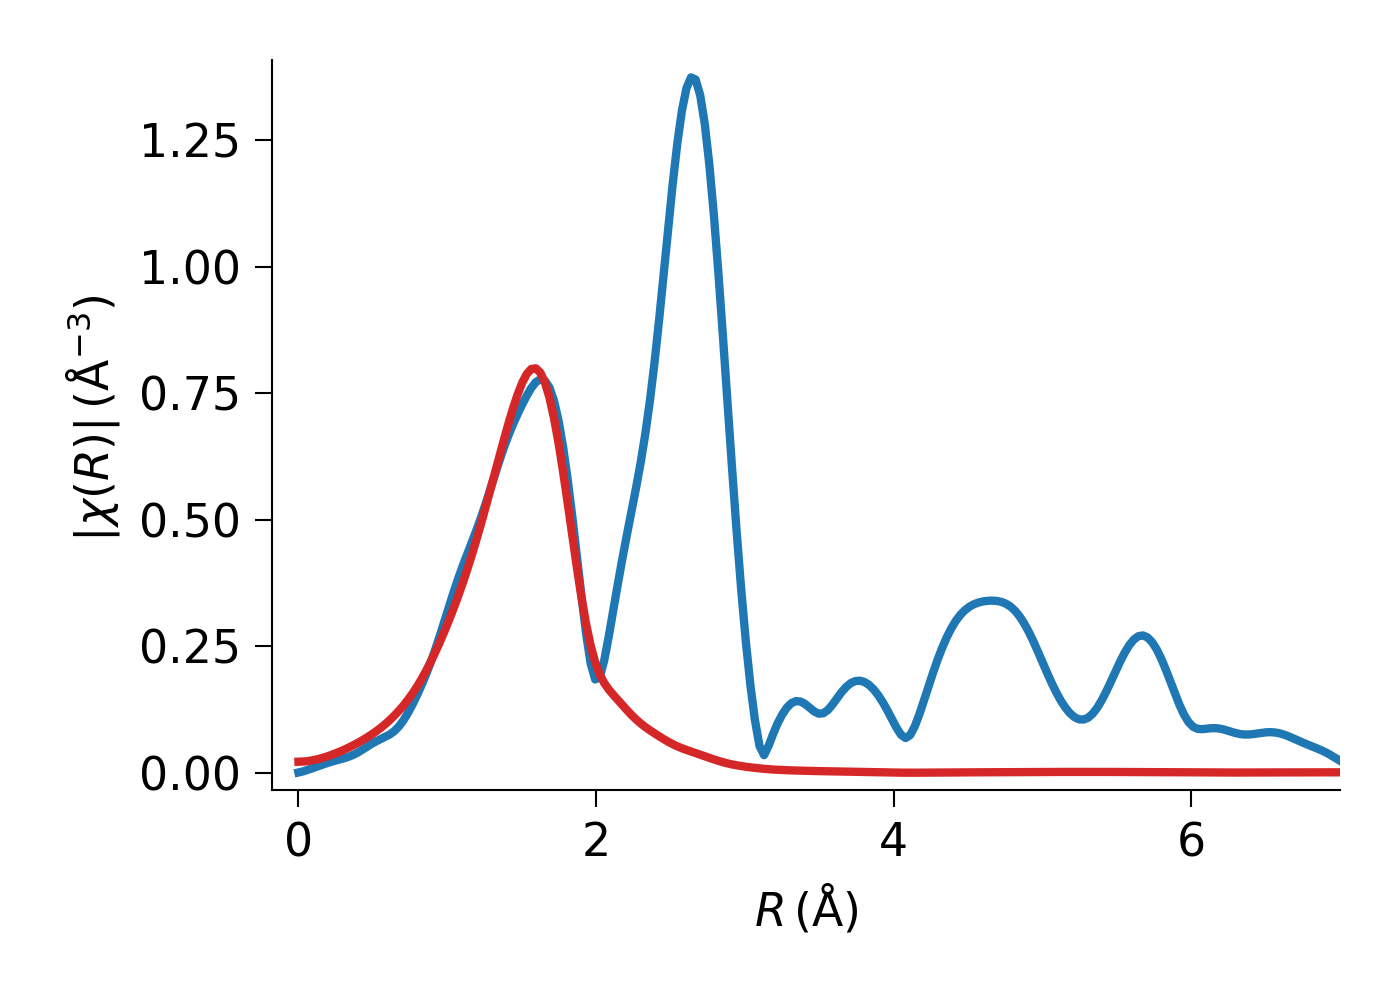
\includegraphics[width=63mm]{figs/fits/feo_1sh_chirmag}

        \vmm
        ${|\chi(R)|}$ for FeO {\Blue{data}} and {\Red{${\rm 1^{st}}$ shell
            fit}}.

      \end{column}
      \begin{column}{35mm}\onslide+<2->
        \setlength{\baselineskip}{10pt} \vmm
        Results:   \vmm
        \begin{tabbing}[ll]\= aaaaa\= aaaaaaaaaaaaaaaa\kill
          \> ${S_0^2}$     \>= 0.7 (fixed)\\
          \> ${N}$           \>= 5.1 ${\pm}$ 0.4\\
          \> ${R}$           \>= 2.09 ${\pm}$ 0.01\AA\\
          \> ${\Delta E_0}$ \>= -1.3 ${\pm}$ 0.9 eV\\
          \> ${\sigma^2}$   \>= 0.012 ${\pm}$ 0.002
          ${\rm\,\AA^2}$.\\
          \end{tabbing}

        \vfill
    \end{column}
  \end{columns}

  \vfill
  \end{cenpage}
\end{frame}

\begin{frame}
\frametitle{Analysis Example:  1st Shell of FeO}
  \begin{cenpage}{135mm}
    \begin{tabular}{ll}
      \begin{minipage}{65mm}
        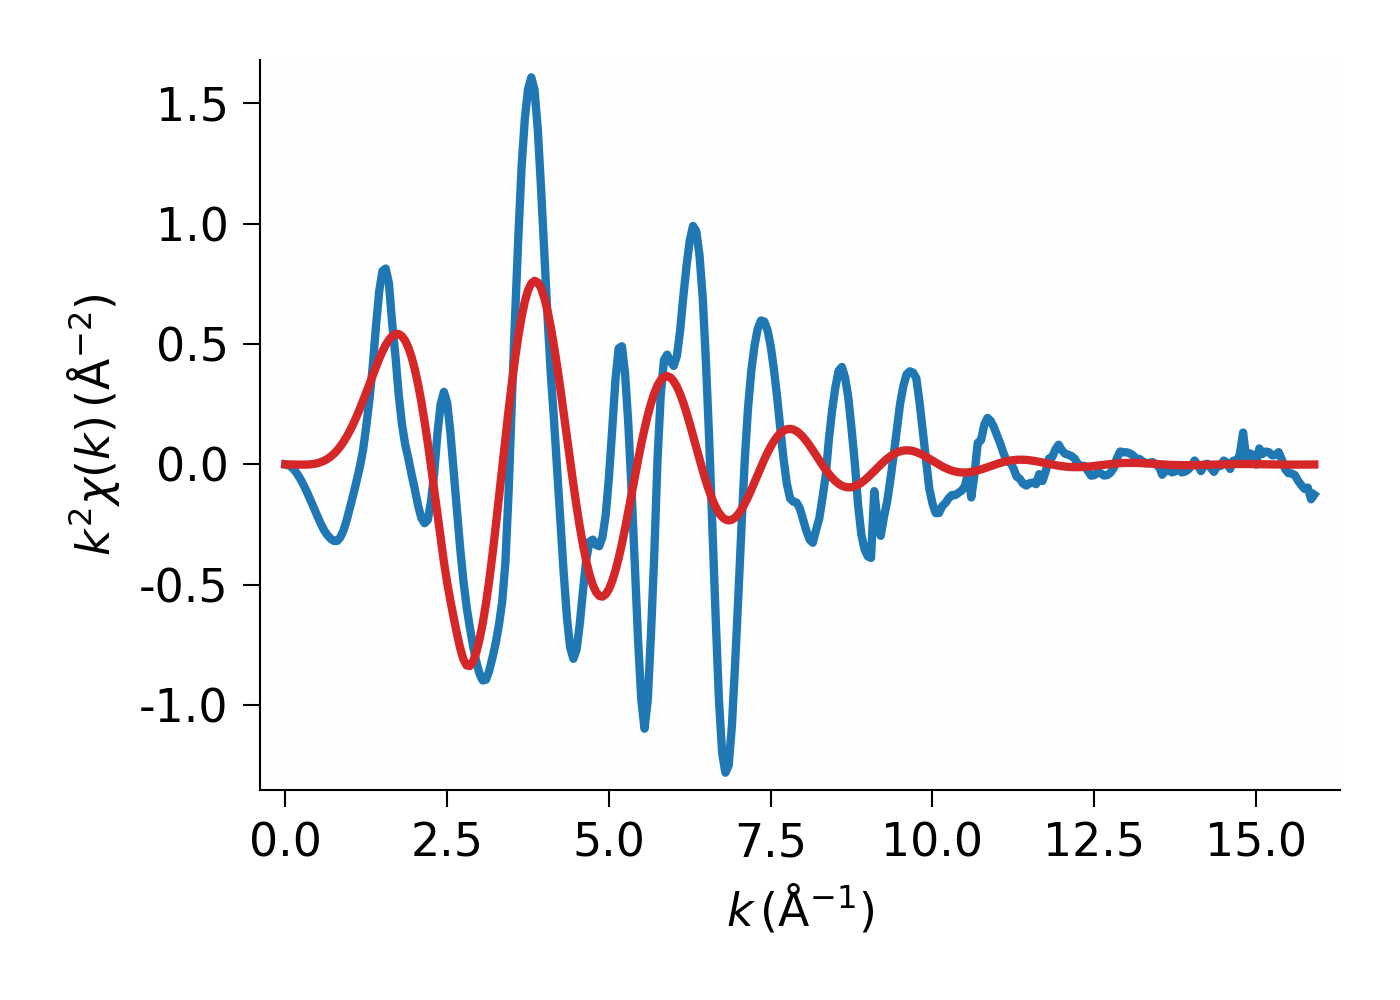
\includegraphics[width=63mm]{figs/fits/feo_1sh_chik}
      \end{minipage}
      &
      \begin{minipage}{55mm}  \setlength{\baselineskip}{10pt}

        {\Red{${1^{st}}$ shell fit in ${k}$ space.}}
        \vmm

        There is clearly another component in the XAFS!
        \vfill
      \end{minipage}
    \\
    \onslide+<2->
      \begin{minipage}{65mm}
        \vspace{-3mm}
        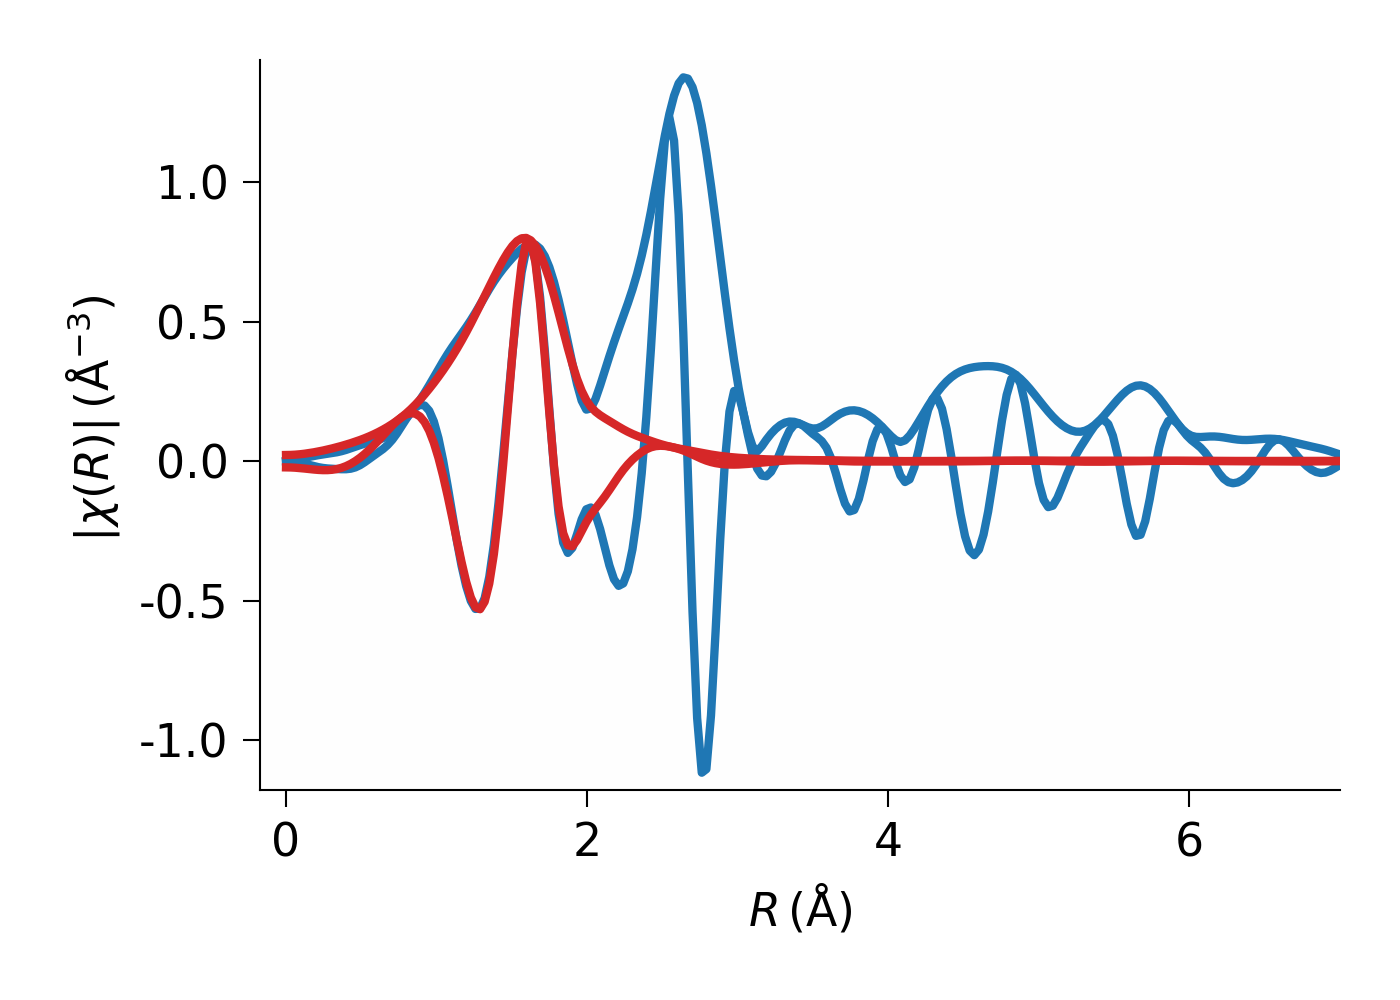
\includegraphics[width=63mm]{figs/fits/feo_1sh_chirre}
      \end{minipage}
      &
    \onslide+<2->
      \begin{minipage}{55mm}  \setlength{\baselineskip}{10pt}
        {\Red{${1^{st}}$ shell fit in ${R}$ space.}}
        \vspace{1mm}

        ${|\chi(R)|}$ and
        {\BlueEmph{${\rm Re[\chi(R)]}$}} for
          FeO (blue), and a ${\rm 1^{st}}$ shell fit (red).  \vspace{1mm}

        Though the fit to the magnitude isn't perfect,
        the fit to ${\rm Re[\chi(R)]}$ looks very good.
        \vfill
      \end{minipage}
  \end{tabular}

  \vfill
    \end{cenpage}
\end{frame}

 \section{Fitting Data}

\begin{slide}{Fitting Strategies}

  Data analysis seeks a {\RedEmph{Model}} that best matches a
  {\BlueEmph{Measurement}}.

  \vmm

  We'll use $\chi^2$ (don't confuse with EXAFS $\chi$!!) to describe how
  good the match is:

  \[ \chi^2  =
  \sum_i^{N_{\rm fit}} \frac{[\chi_i^{\rm measured} - \chi_i^{\rm
      model}({x})]^2}{\epsilon^2}
  \]

  where
  \begin{itemize}
  \item $N_{\rm fit} = $ number of points in the data to fit.
  \item $\epsilon = $ the  estimated noise  level in the data.
  \item $x$  is the set of parameters to be varied in the analysis
  \end{itemize}

  \begin{center}
    {\RedEmph{ The Best Fit is the one with lowest $\chi^2$. }}
  \end{center}

  \vmm   \hrule \vmm

  \onslide+<2->

  Questions:

  \begin{enumerate}
  \item How do I know how many independent measurements I have?
  \item What is $\epsilon$ for my data?
  \item What parameters can/should I vary?
  \end{enumerate}

\end{slide}

\begin{slide}{The Information Content of EXAFS}

\begin{cenpage}{105mm}
    The number of parameters we can reliably extract from our data is limited:
    \vspace{1mm}


    \begin{postitbox}{26mm}
      $\displaystyle  N_{\rm idp} \approx { \frac{2 \Delta k \Delta R}{\pi}}  $
    \end{postitbox}

    \vmm

    where $\Red{ \Delta k}$ and $\Red{ \Delta R}$ are the $k$- and
    $R$-ranges of the usable data.

    \onslide+<2->
    \vmm\vmm

    For a typical range of $k = [3.0, 12.5] \rm\,\AA^{-1}$ and $R = [1.0,
    3.0] \rm\,\AA$, there are $\sim 12$ parameters that can be determined
    from EXAFS.      \onslide+<2-> That's not much!

    \onslide+<2->
    \vmm\vmm

    The Fit statistics and confidence in the measured parameters need to
    reflect this.  But we usually oversample our data ($N_{\rm fit} >
    N_{\rm idp} $) so we have

    \begin{postitbox}{56mm}
      $ \displaystyle
      \chi^2  =  \frac{ N_{\rm idp}}{\epsilon^2 N_{\rm fit}}
      \sum_i^{N_{\rm fit}} [\chi_i^{\rm measured} - \chi_i^{\rm model}({x})]^2
      $
    \end{postitbox}

    Note: I also assumed $\epsilon$ is a constant.

\vfill
\end{cenpage}
\end{slide}


\begin{slide}{Other Fitting Statistics}

  Other ``goodness-of-fit statistics'':
  \vmm

  {\RedEmph{chi-square}}: As before:

  \begin{postitbox}{54mm}  $ \displaystyle
    \chi^2  =  \frac{ N_{\rm idp}}{\epsilon^2 N_{\rm fit}}
    \sum_i^{N_{\rm fit}} [\chi_i^{\rm measured} - \chi_i^{\rm model}({x})]^2
    $
  \end{postitbox}

 \vmm
  {\RedEmph{reduced chi-square}}: scale $N_{\rm varys}$ by the ``degrees of freedom'' :

  \begin{postitbox}{38mm}
    $ \chi^2_\nu =  \chi^2 / (N_{\rm idp}-N_{\rm varys}) $
  \end{postitbox}


  For a ``Good Fit'', $\chi^2_\nu$ should be $\sim$ 1.   This
  {\RedEmph{never}} happens!

\vmm

  {\RedEmph{R-factor}}: $\cal{R}$  gives a ``fractional misfit'' (and
  not scaled by the data  uncertainty $\epsilon$):

\vmm

  \begin{postitbox}{50mm}
    \[
{\cal{R}} = \frac{\sum_i^{N_{\rm fit}}[\chi_i^{\rm measured} -
      \chi_i^{\rm model}({x})]^2 }{
      \sum_i^{N_{\rm fit}} [{\chi_i^{\rm measured}}]^2}
    \]
  \end{postitbox}

\vfill

\end{slide}

%%%%%%%%%%%%%%%%%%%%%%


\section{Uncertainties in $\chi(k)$}
\begin{frame}\frametitle{Propagation of uncertainties in $\chi(k)$}

\begin{cenpage}{95mm}

  Estimating uncertainties in  $\chi(k)$ has always been a challenge.

  \vmm

  We have (by default) estimated the uncertainty in $\chi(k)$ as
  {\BlueEmph{white noise}} {\tiny{(Newville, Boyanov, and Sayers, {\emph{J
          Synch Rad}}, 1999)}}, using $\chi(R)$ between [15, 25] \AA.

\end{cenpage}

\begin{columns}
  \begin{column}[T]{60mm}

    {\onslide+<1->  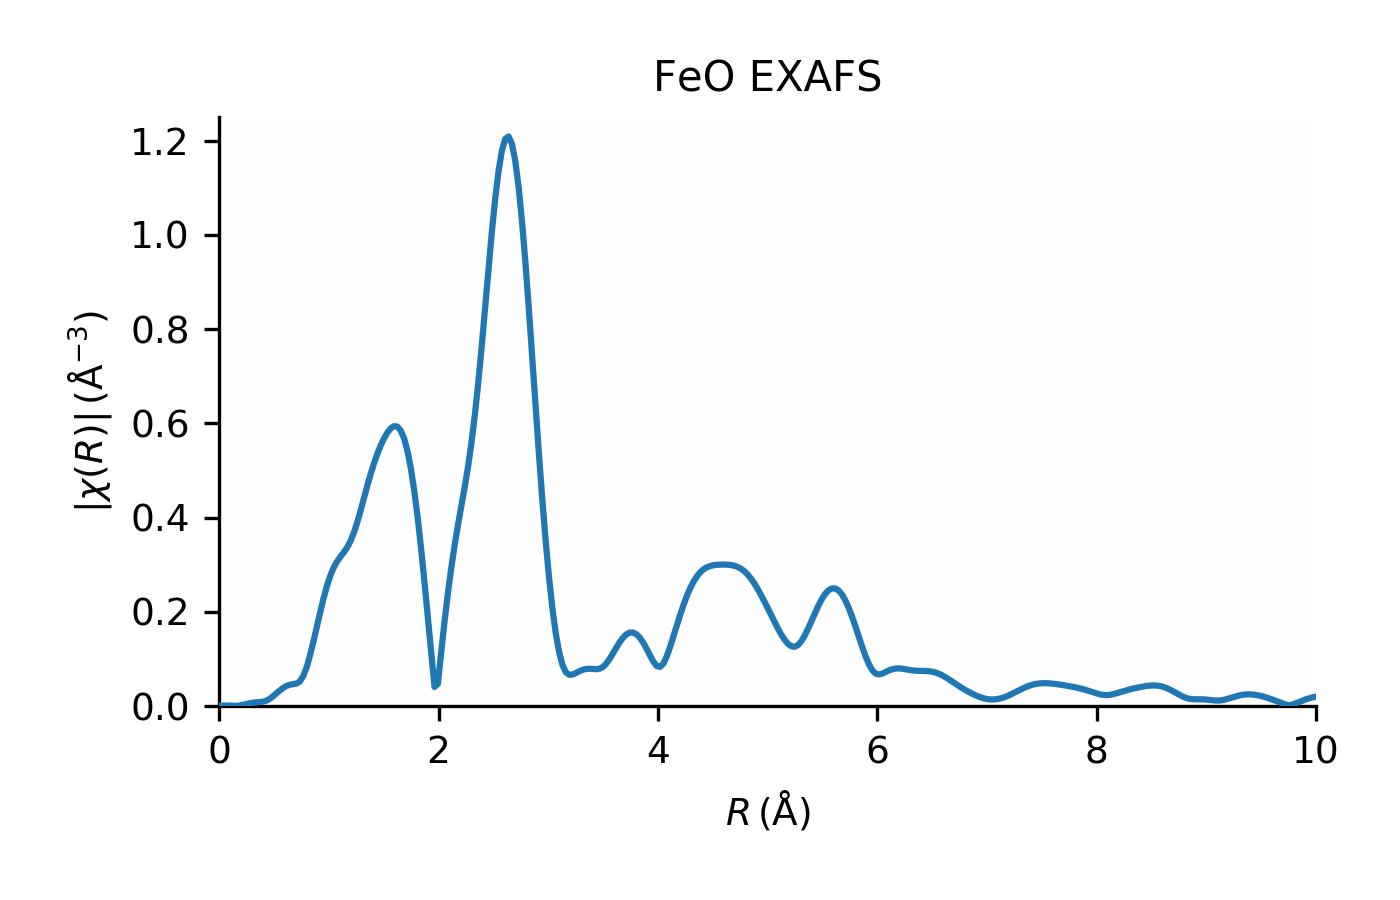
\includegraphics[width=60mm]{figs/errors/feo_chir}  }


  \end{column}
  \begin{column}[T]{60mm}

    {\onslide+<2-> 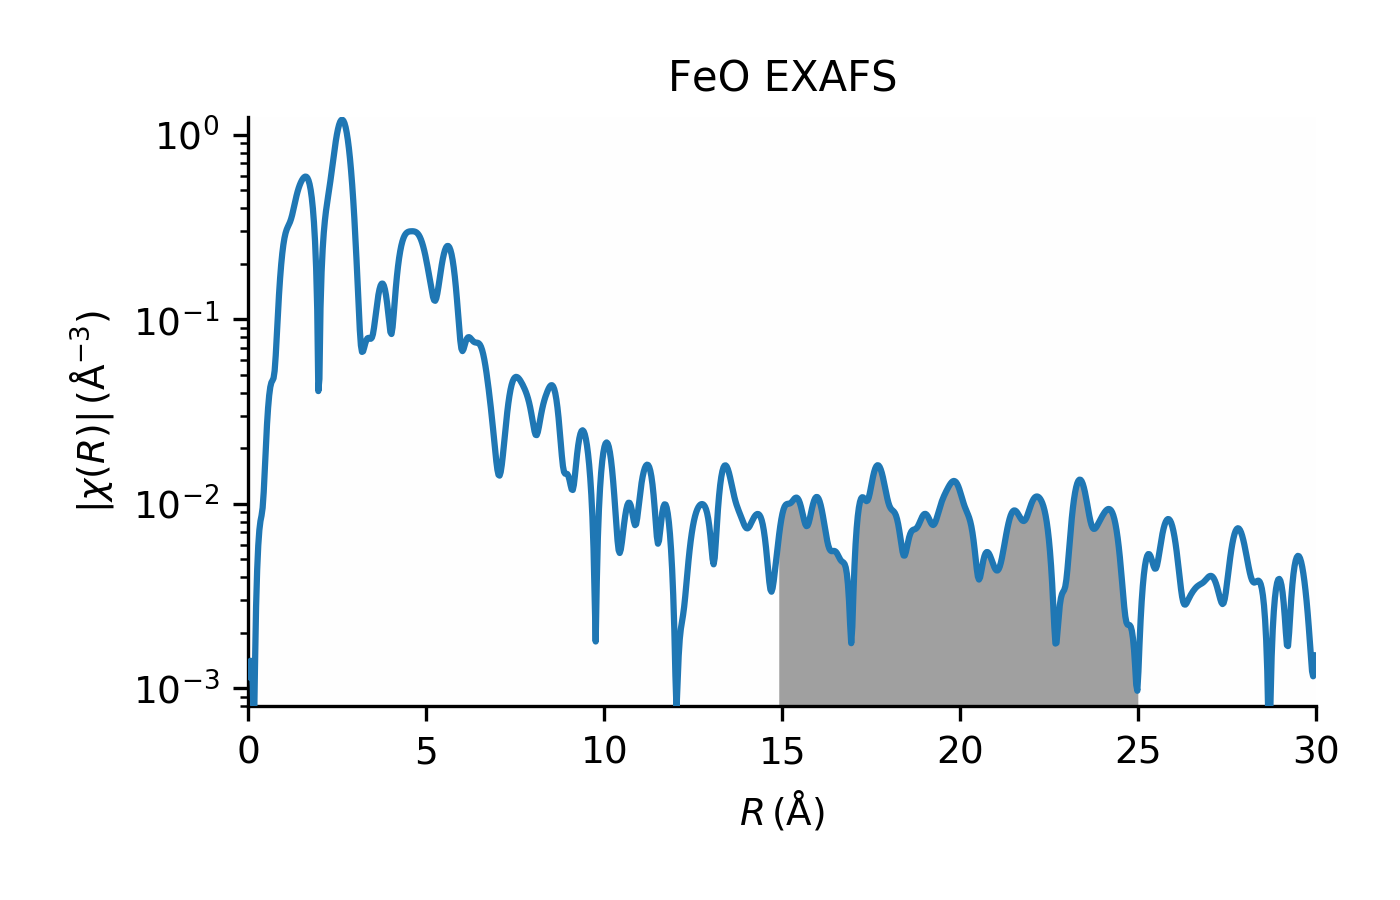
\includegraphics[width=60mm]{figs/errors/feo_chir_logscale} }

  \end{column}
\end{columns}

{\onslide+<2->

  \begin{cenpage}{105mm}


    The ``high-R'' portion of $\chi(R)$ can estimate the
    ``white noise'' in the data pretty well.

    \vmm
    This is easy to do, but we know it misses an important component:
  \end{cenpage}


  \begin{postitbox}{63mm}
      {uncertainties from  background subtraction}
  \end{postitbox}

}

\end{frame}


\begin{frame}\frametitle{ Uncertainties in $\chi(k)$ from background subtraction}


\vmm
\begin{cenpage}{105mm}

  We can propagate the uncertainties from the fit of the background spline
  to estimate the uncertainty in $\chi(k)$ from the background subtraction.

  \vmm \vmm

  This is {\BlueEmph{not white noise}}.   In fact, it tends to have a peak
  somewhat above $2 R_{\rm bkg}$
\end{cenpage}

\begin{columns}
  \begin{column}[T]{60mm}

    {\only<1> { 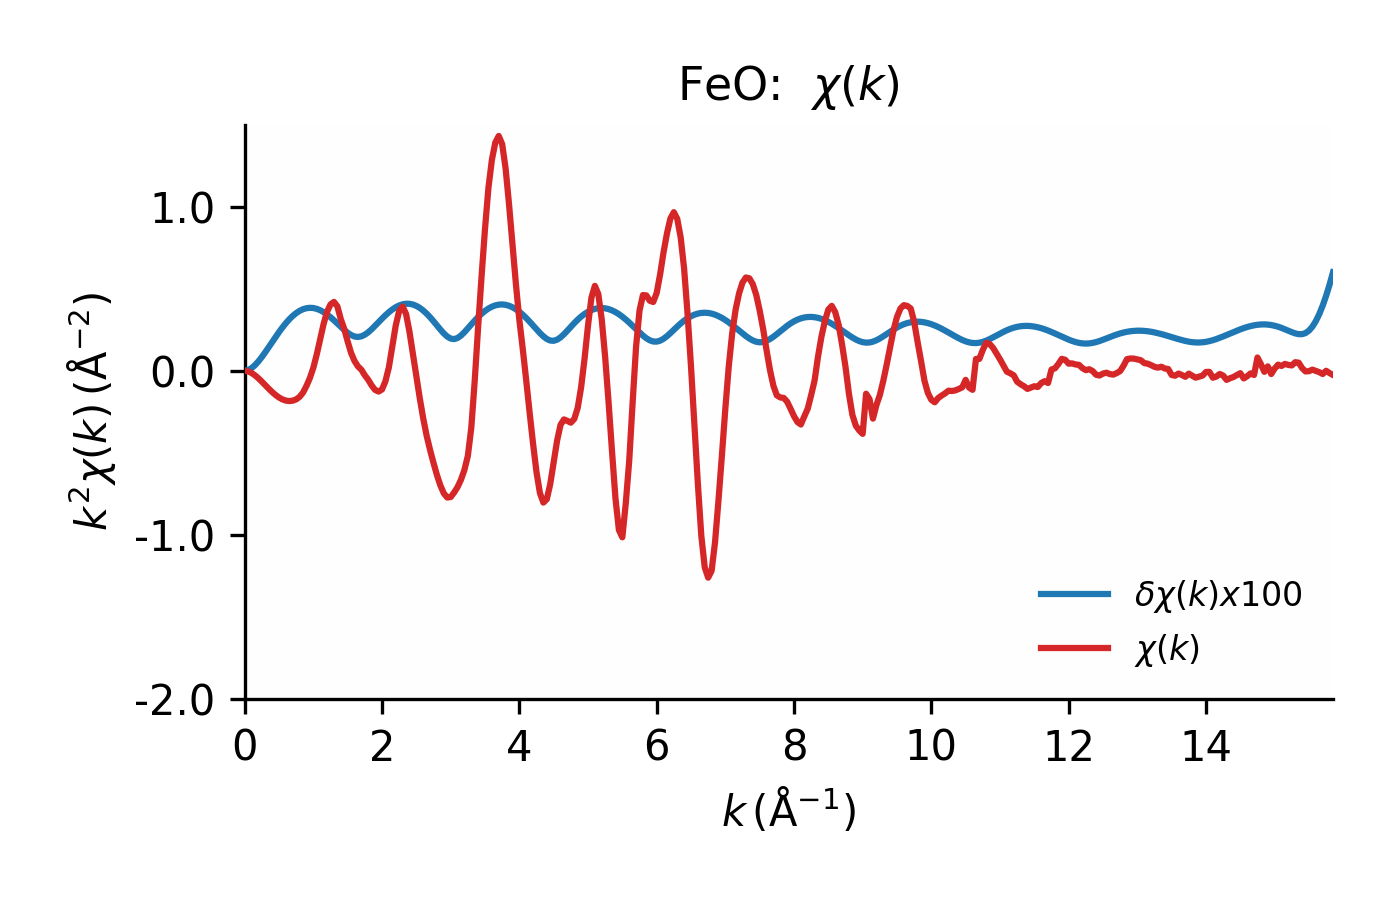
\includegraphics[width=60mm]{figs/errors/feo_chik_deltachi}}}

    {\only<2,3> { 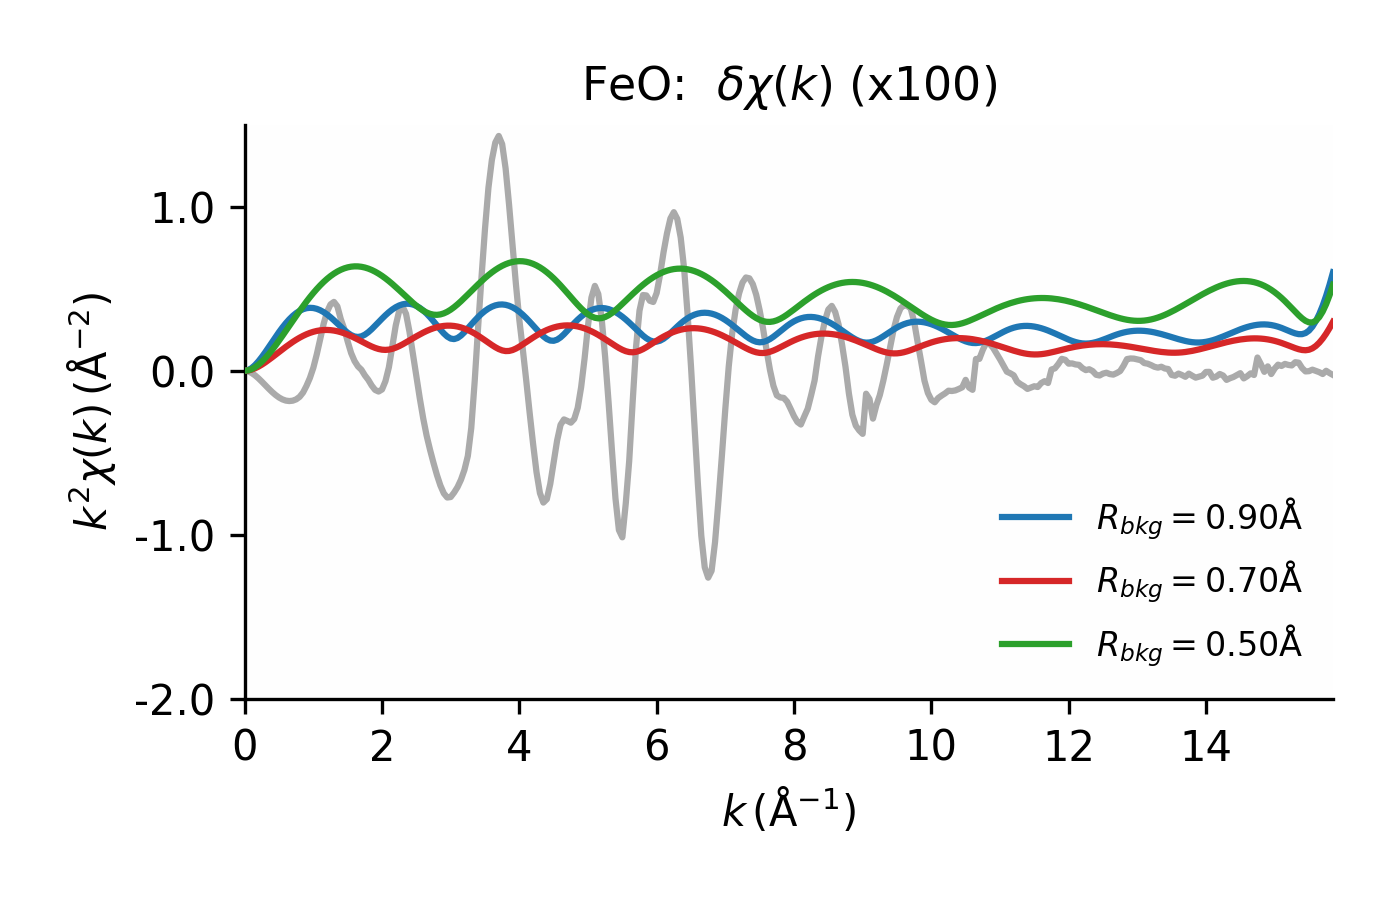
\includegraphics[width=60mm]{figs/errors/feo_deltachik_rbkg} }}

    \end{column}

    \begin{column}[T]{60mm}

      {\only<1>{ 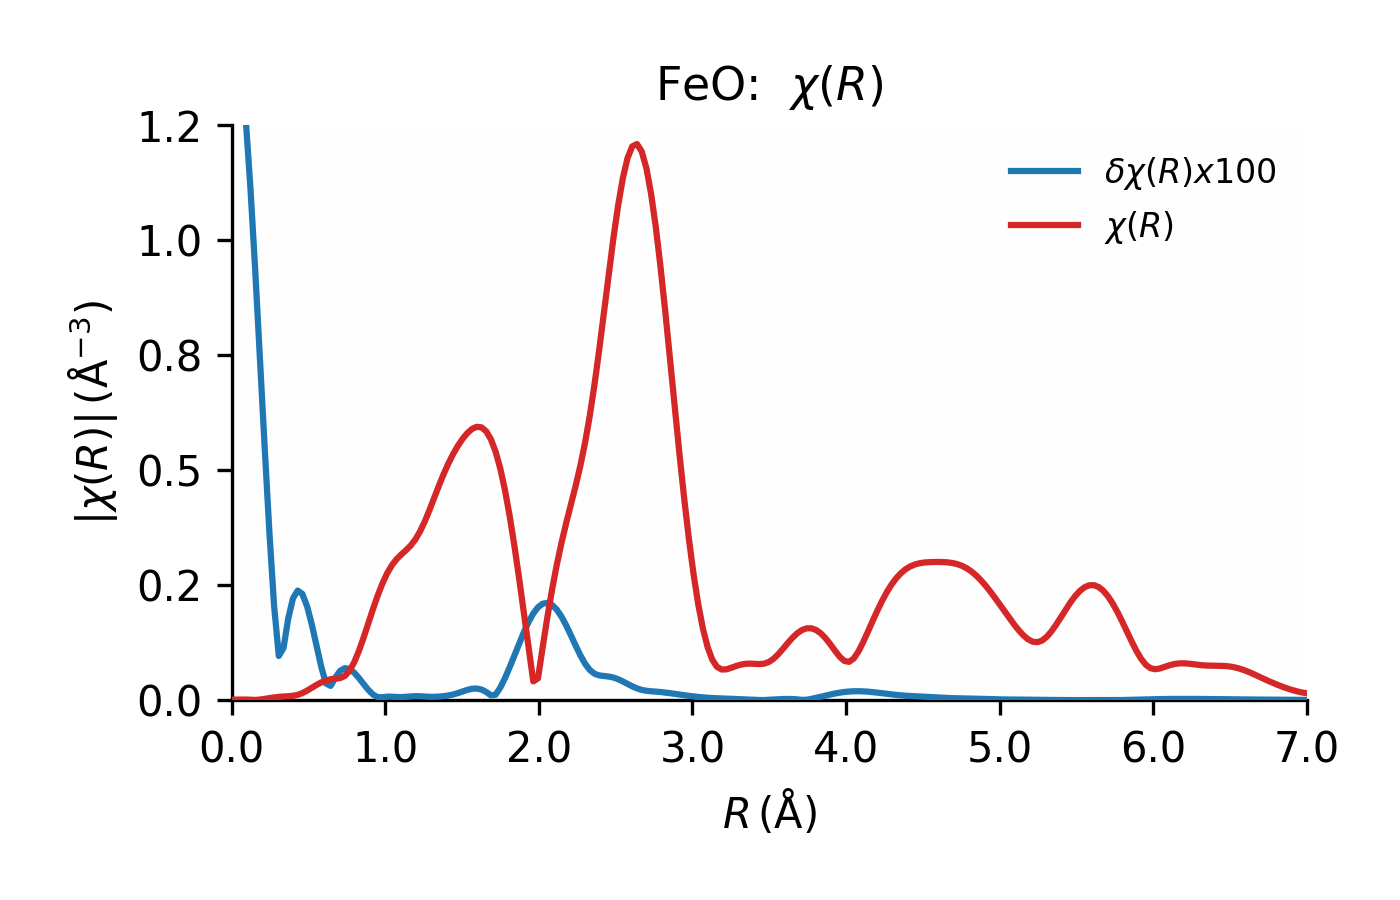
\includegraphics[width=60mm]{figs/errors/feo_chir_deltachi} }}

      {\only<2,3>{ 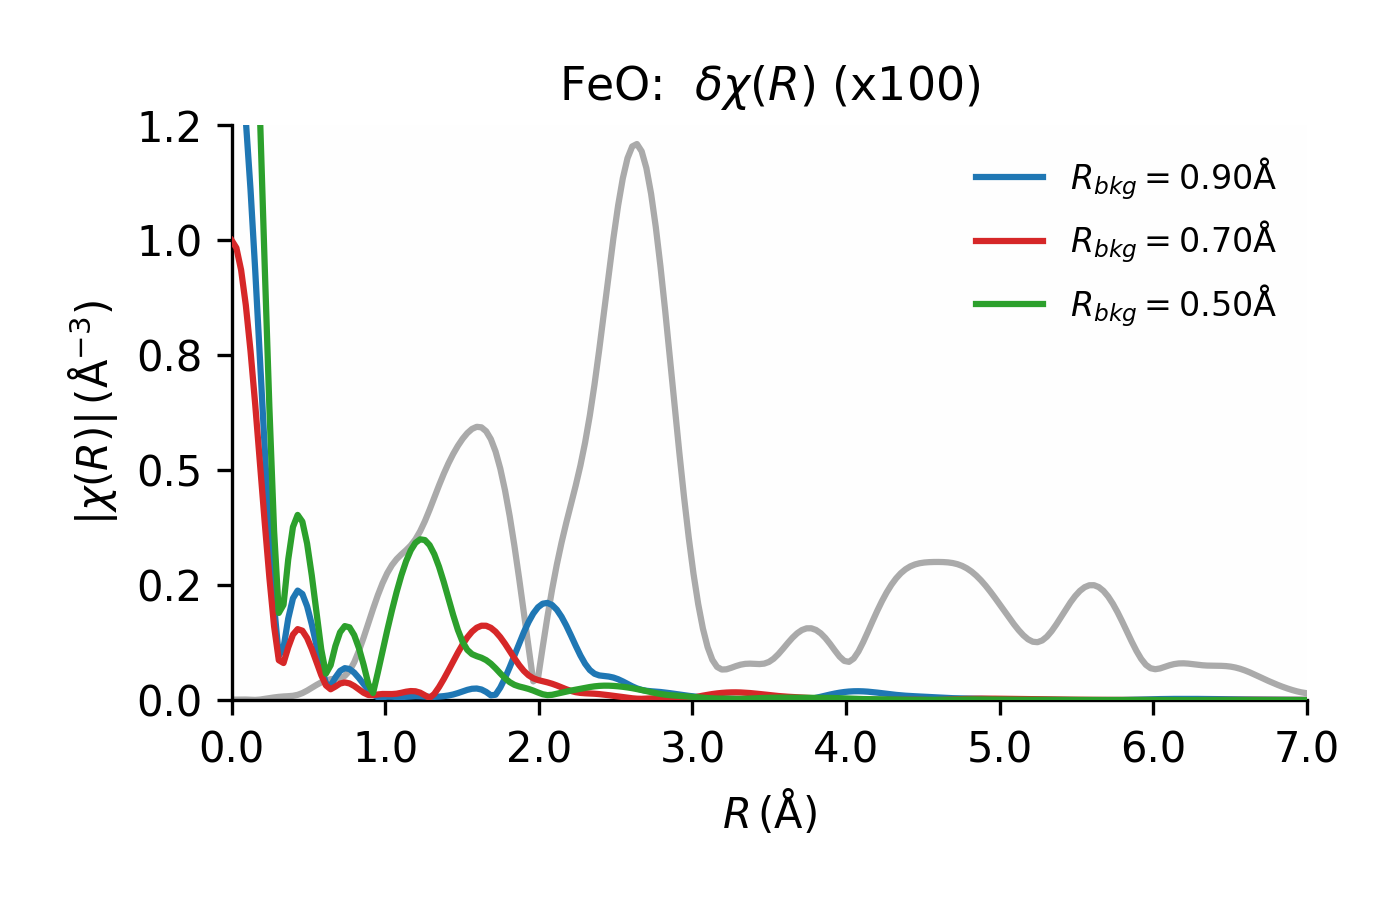
\includegraphics[width=60mm]{figs/errors/feo_deltachir_rbkg} }}

    \end{column}

\end{columns}

\vmm

{\onslide+<3-> {

\begin{cenpage}{105mm}

    Using this $\delta\chi(k)$ array reduces the $\chi^2$
    statistic by $2\times$ or  more.

\end{cenpage}

}}


\end{frame}

%%%%%%%%%%%%%%%%%%%%%%
\begin{slide}{Error Bars: the uncertainties in the fit variables}

\begin{cenpage}{95mm}
A fit finds a set of values $\Blue{x_0}$ that are the ``best fit'' of the variables
$\Blue{x}$ -- they give the lowest value of  $\chi^2$.

\begin{center} Uncertainties in $\Blue{x}$ are estimated by increasing the
  $\chi^2$ by 1: \end{center}

\end{cenpage}

\begin{columns}
\begin{column}{58mm}

\onslide+<2->

 \wpdf{58mm}{figs/errors/ellipse}

\end{column}
\begin{column}{55mm}

{\onslide+<2->
Some Parameters are {\RedEmph{Correlated}}:

\vmm

Changing {\Blue{$x$}} away from its best value will change the best value
for {\Blue{$y$}}.

\vmm

\begin{postitbox}{53mm}
  For EXAFS, ($R$, $E_0$) and ($N$, $\sigma^2$) are usually very highly
  correlated ($>0.85$).
\end{postitbox}
\vmm
}
\end{column}
\end{columns}

 \onslide+<2-> \vmm
 {\RedEmph{Increasing $\chi^2$ by 1 assumes we have a ``Good Fit'', with $\chi^2_\nu \approx 1$}}.

 \vmm We typically have  $\chi^2_\nu \gtrsim 50$  (Actually, we  {\emph{can
     now do better}}!).

\vmm
We increase the best $\chi^2$ by $\chi^2_\nu$ to estimate error bars.


\vmm \vmm

\end{slide}

% %%%%%%%%%%%%%%%%%%%%%%
% \begin{slide}{Error Bars: correlations between fit variables}


%     Pairs of variables can be {\RedEmph{correlated}}: changing one variable away
%     from its optimum value can be compensated by changing another variable away
%     from its best value.  The uncertainties needs to take correlations into
%     account.

%     \vmm\pause

%     \begin{center} \wpdf{50mm}{figs/errors/ellipse2}   \end{center}

%     \vmm
%     The uncertainty in $x$ is $\delta x$, NOT  $\delta x'$!

%     \vmm

%     The correlation between variables is given by the slope of the ellipse:

%     \begin{postitbox}{75mm}    how much does $y$ want to change when
%       changing $x$?
%     \end{postitbox}

%     \vmm

% \vfill
% \end{slide}

 \begin{slide}{Fitting in $R$- or $k$-space:  What do we model?}

  The $\chi^2$ definition didn't say anything about what our data
  $\chi_i^{\rm measured}$ actually is \ldots

  \onslide+<2->
  \vmm  We usually fit in $R$-space, so that  we can select which
  ``shells'' to ignore:

  \vmm \vmm

  \begin{columns}
    \begin{column}{53mm}  \wgraph{53mm}{reduction/chik}  \end{column}
    \begin{column}{53mm}  \wgraph{53mm}{reduction/chir_win}  \end{column}
  \end{columns}

  \vmm \onslide+<3-> Fitting $\chi(R)$ (both real and imaginary parts!) gives more
  meaningful fit statistics -- we know that we're not fitting all the
  spectral features.

  \vmm \onslide+<4->

  {\RedEmph{Plus:}}    We can have $\chi_i^{\rm measured}$  extend over

  \begin{center}{\Red{multiple data sets}}, {\Red{multiple $k$-weightings}},  etc, \end{center}

  as long as we generate the corresponding {\Red{$\chi_i^{\rm model}(x)$}} to
  match these data.

\vfill
\end{slide}


 

\begin{slide}{EXAFS Analysis: Second Shell of FeO}

  Adding the 2nd shell Fe -- {\file{feffNNNN.dat}} for Fe-Fe -- and
  refining {\Blue{${R}$}}, {\Blue{${N}$}}, {\Blue{${\sigma^2}$}}:

    \vspace{1mm}

    \begin{tabular}{ll}
      \begin{minipage}{55mm} {\wpdf{54mm}{figs/fits/feo_r_2sh_mag}}
      \end{minipage}
      &
      \begin{minipage}{49mm}
        \vspace{1mm}

        ${|\chi(R)|}$ data for FeO (blue), and fit of ${\rm
          1^{st}}$ and ${\rm 2^{nd}}$ shells (red).  \vfill
        \vspace{1mm}

        These
        results are consistent with the known values for FeO:\par
         6 O at 2.14\AA, 12 Fe at 3.03\AA.
    \end{minipage}
  \end{tabular}

  \onslide+<2->{
  Fit results:     \hspace{6mm} Statistics: $R \approx 0.011 $
 \hspace{5mm}  $\chi^2_\nu \approx 4 $.

  \begin{center}
    \begin{tabular}{|c|rrrr|}
    \hline
    Shell & ${N}$ & ${R}$ (\AA) & ${\sigma^2}$
    (${\rm\AA^2}$) & ${\Delta E_0}$ (eV) \\
    \hline
    Fe-O  &  4.9(0.8) & 2.11(.01) & 0.011(.002) & {\Red{0.7(0.9)}}\\
    Fe-Fe & 11.6(1.4) & 3.07(.01) & 0.013(.002) & {\Red{0.7(0.9)}}\\
    \hline
  \end{tabular}
  \end{center}

  \vmm

  }
  \onslide+<3-> {
  These are typical even for a ``very good fit'' on known structures.

  The calculation for ${{\Red{f(k)}}}$ and
  ${{\Red{\delta(k)}}}$ are good, but not perfect!
}


\vfill
\end{slide}

\begin{slide}{EXAFS Analysis: Second Shell of FeO}

  Other views of the data and fit:

    \begin{tabular}{ll}
      \begin{minipage}{55mm} {\wpdf{55mm}{figs/fits/feo_k_2sh}}
      \end{minipage}
      &
      \begin{minipage}{53mm}  \setlength{\baselineskip}{11pt}
        The Fe-Fe EXAFS extends to higher-$k$ than the Fe-O EXAFS.

        \vmm Even in this simple system, there is some
        {\RedEmph{overlap}} of shells in ${R}$-space.

        {\onslide+<2->
          \vmm The fit in ${\rm Re[\chi(R)]}$ look especially
          good -- this is how the fits are done.

          \vmm
          }

    \end{minipage}
    \\
    \begin{minipage}{55mm}
      {\wpdf{55mm}{figs/fits/feo_r_2sh_paths}}
    \end{minipage}
    &
    \onslide+<2->{
      \begin{minipage}{55mm} {\wpdf{55mm}
          {figs/fits/feo_r_2sh_cmplx}}
      \end{minipage}}
  \end{tabular}

\vfill
\end{slide}

\section{Path Parameters}
 
\begin{slide}{Path Parameters: what can we vary in a fit?}

\begin{cenpage}{108mm}
  The EXAFS Equation has at least 4 adjustable parametes {\RedEmph{Per
      Path}}:
  $E_0$, $NS_0^2$, $R$, and $\sigma^2$.  \hspace{5mm}     But $N_{\rm idp}$  is low:

  \[ N_{\rm idp} = 8 \> \> \>
  {\rm for} \> \Delta R = 1 \, {\rm \AA} \>\> {\rm and} \>\> \Delta k = 12.5\,
  {\rm \AA^{-1} } \]

  \vmm\onslide+<2->

  For simple crystalline structures with well-isolated, single-scattering
  path (like FeO), it's OK to fit $N$, $R$, $\sigma^2$, and $E_0$ for every
  path.

  \vmm

  For more complicated problems, we need a way to limit the number of
  parameters varied.

  \vmm

  We might {\emph{want}} to impose relationships between parameters to get
  more meaningful results\ldots


\end{cenpage}
\vfill
\end{slide}



\section{Parameters and Constraints}
 \subsection{Constraints and Generalized Variables}
\begin{frame}[fragile] \frametitle{Constraints and Generalized Variables}

  Instead of varying the Path Parameters directly, we write them in terms of
  {\RedEmph{Generalized Variables}}.  This allows simple {\RedEmph{Constraints}} and model building:

\begin{columns}
  \begin{column}{53mm}

  \begin{CodeBlock}{50mm}{Parameter=Variable}
{\Blue{\# one variable e0 for 2 paths}}
{\Red{params = group(e0 = guess(1.0), \ldots)}}

path1  = feffpath('feo.dat', {\Red{e0='e0'}})
path2  = feffpath('fefe.dat', {\Red{e0='e0'}})
  \end{CodeBlock}
  \hspace{1mm}   \vmm

  \onslide+<2->
  \begin{CodeBlock}{50mm}{Mixed Coordination Shell}
{\Blue{\# mix O and S in 1st coordination shell}}
params = group(s02   = param(0.80, vary=False),
               sfrac = guess(0.5))

path1 = feffpath('feo.dat', {\Red{s02='s02*sfrac'}})
path2 = feffpath('fes.dat', {\Red{s02='s02*(1-sfrac)'}})
  \end{CodeBlock}

  \vmm

  \end{column}
  \begin{column}{57mm}
    \onslide+<3->
  \begin{CodeBlock}{55mm}{Einstein Temperature }
{\Blue{\# Use 1 ``theta'' to set sigma2 for multiple paths}}

params = group(amp=param(1, vary=True),
               theta=param(250, min=0, vary=True), \ldots)

path1_100K = feffpath('fefe.dat', s02='amp', \ldots,
                      sigma2='sigma2_eins(100, theta)')

path1_200K = feffpath('fefe.dat', s02='amp', \ldots,
                      sigma2='sigma2_eins(200, theta)')

path1_300K = feffpath('fefe.dat', s02='amp', \ldots,
                      sigma2='sigma2_eins(300, theta)')

  \end{CodeBlock}\\
\end{column}
\end{columns}

\vmm This allows us to use {\BlueEmph{Prior  Knowledge}} into the data analysis, and
consider more complicated problems:

\vfill

  \begin{itemize}
  \item force one $R$ for the same bond for data taken from different
    edges.

  \item model complex distortions (height of a sorbed atom above a surface).
  \end{itemize}


\end{frame}

% \begin{slide}{Constraints, Generalized Variables examples}


%   Constraints and Generalized Variables are one kind of ``Prior
%   Knowledge'',  allowing us to build and compare simple physical models for
%   our data.

%   \vmm   This allows us to consider more complicated problems:

%   \vmm

%   {\Red{
%       \begin{tabular}{clcl}
%         &multiple neighboring species  &&  multiple sites for central atom \\
%         &multiple scattering paths     &&  multiple polarizations \\
%         &multiple data sets            &\hspace{4mm}&  multiple edges to co-refine   \\
%       \end{tabular}
%     }}

%   \vmm Other constraints:

%   \begin{itemize}
%   \item force one $R$ for the same bond for data taken from different
%     edges.

%   \item model complex distortions (height of a sorbed atom above a surface).
%   \end{itemize}

% \vfill
% \end{slide}

 
%%%%%%%%%%%%%%%%%%%%%%
\subsection{Example: Cu metal at 3 temperature}
\begin{frame}[fragile] \frametitle{Example: Cu metal at 3 temperature}


    A very simple example of a Multi-Data-Set Fit:

    Cu metal, at 3 different  temperatures: 10K, 50K 150K.

   \begin{columns}
     \begin{column}{48mm}
        \vmm  Path Parameters:
       \begin{itemize}
       \item $E_0$:  Same for all $T$
       \item $S_0^2$  Same for all $T$
       \item $R$:  expands linearly with $T$ (slope + offset).
       \item $\sigma^2$:  goes as Einstein temperature (as before).
       \end{itemize}

       {\RedEmph{12 parameters become 5.}}

       \vmm Fit range: \vmm

       \hspace{2mm} $R = [1.60, 2.75] \rm\, \AA$

       \vmm
       \hspace{2mm}  $k = [1.50, 18.50] \rm\, \AA^{-1}$
     \end{column}
     \begin{column}{53mm}

  \begin{CodeBlock}{55mm}{Cu at three temperatures}

# define fitting parameter group
pars = group(amp      = param(1, vary=True),
             del_e0   = guess(2.0),
             theta    = param(250, min=10, vary=True),
             dr_off   = guess(0),
             dr_slope = guess(0) )

# define 3 Feff Path, give expressions for Path Parameters
path1_10  = feffpath('feff0001.dat',
                     s02='amp', e0='del_e0',
                     deltar='dr_off + 10*dr_slope',
                     sigma2='sigma2_eins(10, theta)')

path1_50  = feffpath('feff0001.dat',
                     s02='amp', e0='del_e0',
                     deltar='dr_off + 50*dr_slope',
                     sigma2='sigma2_eins(50, theta)')

path1_150 = feffpath('feff0001.dat',
                     s02='amp', e0='del_e0',
                     deltar='dr_off + 150*dr_slope',
                     sigma2='sigma2_eins(150, theta)')

   \end{CodeBlock}
 \end{column}
\end{columns}

\end{frame}


%%%%%%%%%%%%%%%%%%%%%%
\subsection{Example: Cu metal Results}
\begin{frame}[fragile] \frametitle{Example: Cu metal Results}

  \begin{tabular}{ll}
    \begin{minipage}{50mm}
      \begin{tabular}{lll}
        {\ } &{\tt{amp}}  &   $0.91(0.08)$ \\
        &{\tt{theta}}  &   $233.5(19.6) \rm\, K $ \\
        &{\tt{del\_e0}}  &   $0.4(1.3) \rm \, eV$ \\
        & {\tt{dr\_off}} &   $0.002(0.003) \rm \, {\AA}/K $ \\
        &{\tt{dr\_slope}}   &    $0.5(1.8)\times 10^{-5} \rm \, {\AA}$ \\
      \end{tabular}
  \vmm
\end{minipage} &
\begin{minipage}{50mm}
  \wpdf{49mm}{figs/Cu3temp/cu_3temp_mag10}
\end{minipage} \\
\begin{minipage}{50mm}
  \wpdf{49mm}{figs/Cu3temp/cu_3temp_50}
\end{minipage} &
\begin{minipage}{50mm}
  \wpdf{49mm}{figs/Cu3temp/cu_3temp_150}
\end{minipage}\\
\end{tabular}
\end{frame}

%%%%%%%%%%%%%%%%%%%%%%
% \begin{slide}{Room Temperature Cu Fit }

%   Simple fit to first shell of Cu foil (300K): $k = [2,16] \rm\,
%     \AA^{-1}$, $R = [1.7,2.6] \rm\, \AA$, $k$-weight=2, $N_{\rm idp} = 8.4
%     $.  Fit results and statistics:


%     {
%       \hspace{0.1mm}\begin{tabular}{lll}
%         $R = 2.548(0.007) \, \rm\AA$
%         &
%         $\Delta E_0 = 4.5(0.6)$
%         &
%         $C_3      = 9(9) \times10^{-5} \rm\, \AA^3$
%         \\
%         $\epsilon_k = 1.6 \times 10^{-4}$
%         &
%         $S_0^2 = 0.96(0.04)$
%         &
%         $\sigma^2 = 8.5(0.3) \times10^{-3} \rm\, \AA^2$
%         \\
%         $\chi^2 = 678$ &
%         $\chi^2_\nu = 196.7$   & ${\cal{R}} = 0.00107 $\\
%       \end{tabular}
%     }

%     \vmm
%       \begin{tabular}{lcl}
%         \wgraph{49mm}{errors/cufit02} & \hspace{2mm} &
%         \wgraph{49mm}{errors/cufit01} \\
%       \end{tabular}

%       \begin{itemize}
%       \item ${\cal{R}} = 0.1\% $ -- a good fit!  But like $\chi^2_\nu$,
%         ${\cal{R}}$ is larger than the $\epsilon_k$ suggests.
%       \item These error bars account for correlations.  They increase
%         $\chi^2$ by $\chi^2_\nu$ (not 1), which scales them by
%         $\sqrt{\chi^2_\nu}\approx 14$ over ``increase $\chi^2$ by 1''.
%       \end{itemize}

%       \vmm
% \vfill
% \end{slide}


\section{Disorder Terms}


\begin{slide}{Structural Disorder and the Pair Distribution Function}

  \begin{cenpage}{135mm}

  An EXAFS measurement averages billions of {\BlueEmph{snapshots}} of the
  local structure:

\begin{cenpage}{88mm}
\begin{itemize}
\item Each absorbed x-ray generates 1 photo-electron.
\item the photo-electron / core-hole pair lives for about
  $10^{-15}$ s --  much faster than the thermal vibrations ($10^{-12}$ s).
\item An EXAFS measurement samples $10^4$ (dilute fluorescence) to $10^{10}$
  absorbed x-rays for each energy point.
\end{itemize}
\end{cenpage}

\vmm
 \vmm

So far, we've put this in the EXAFS Equation as \hspace{2mm}
$\chi \sim N \exp({-2k^2\sigma^2}) $

\vmm \hrule \vmm \onslide+<2->

\begin{columns}
  \begin{column}{70mm}
    More generally, EXAFS samples the

    \vmm
    {\RedEmph{Partial Pair Distribution Function}}

    \vmm

    {\RedEmph{$g(R)$}} =   probability that an
    atom is a distance $R$ away from the absorber.

    \vspace{8mm}

    \end{column}
  \begin{column}{65mm}

    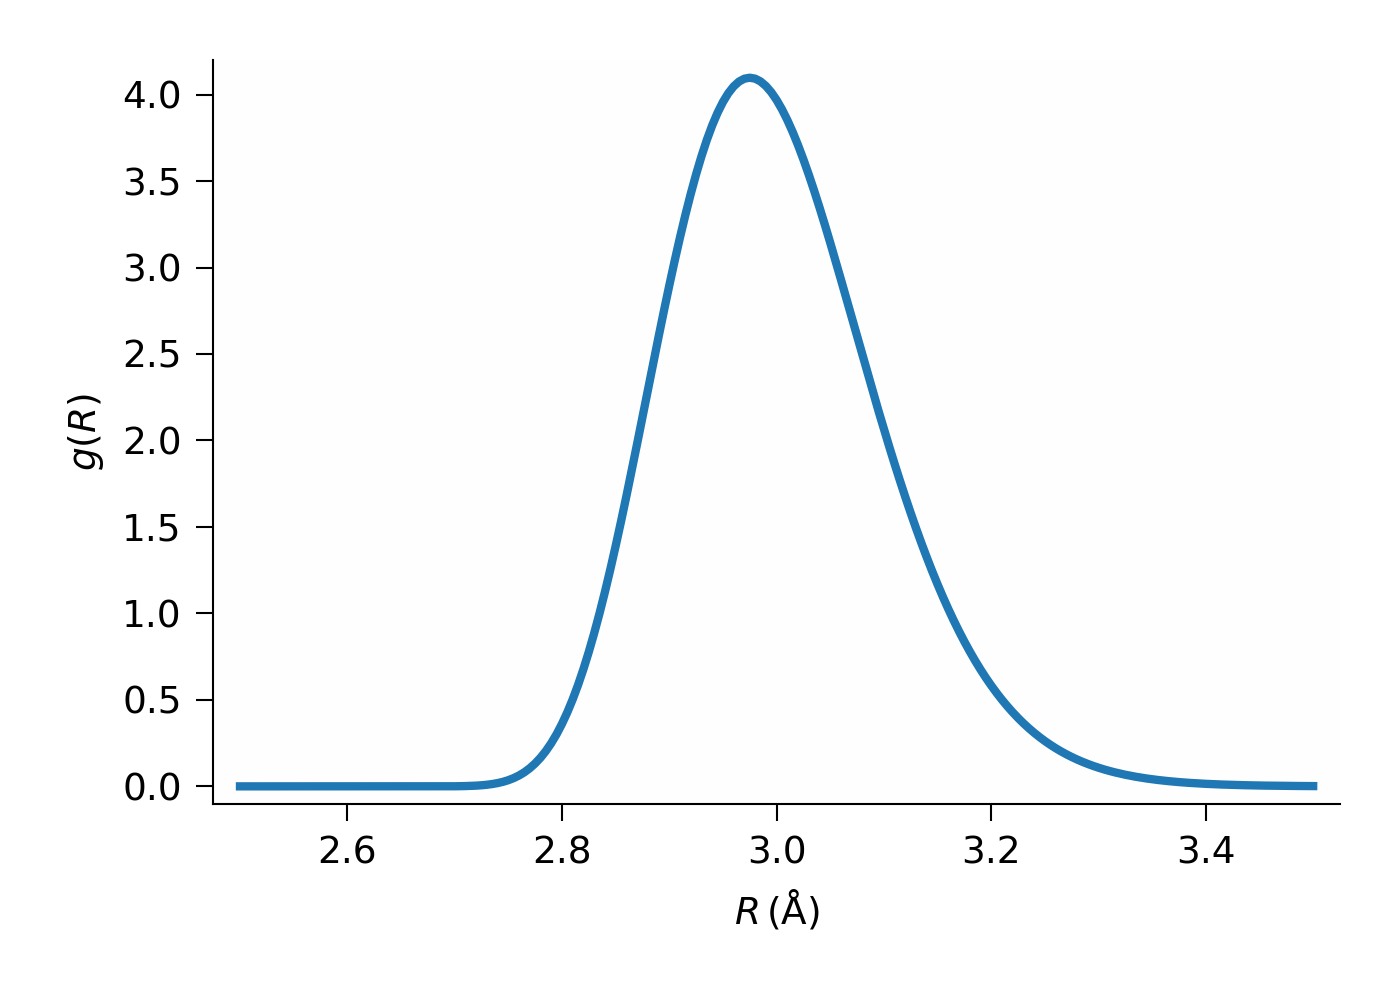
\includegraphics[width=60mm]{figs/errors/gnxas}
    \end{column}
  \end{columns}
\end{cenpage}
\end{slide}


\begin{slide}{EXAFS and The Pair Distribution Function}


  \begin{cenpage}{135mm}
  To fully account for a highly disordered local structure, we should use

\[
    \chi(k)  = \Biggl\langle \sum_j {\frac{f_j(k)e^{i2kR_j + \delta_j(k)}}{kR_j^2}} \Biggr\rangle
\]

where $ \langle x \rangle = \int dR\, x \, g(R) / \int dR\, g(R) $ --
averaging over the billions+ of snapshots.

\vmm\pause
$R$ won't change too much, so we'll neglect the changes to $1/R^2$:

\[
  \chi \approx
  \sum_j {f_j(k){\frac{e^{ i\delta_j(k)} }{kR_j^2}}}   \biggl\langle e^{i2kR_j}  \biggr\rangle
\]

each path in the sum now has a $g(R)$ with respect to the absorbing atom.

\vmm \hrule \vmm \onslide+<3->

The {\RedEmph{the cumulant expansion}} relates $\langle e^x\rangle$ to $\langle x \rangle$, the moments of $g(x)$:


\[ \biggl\langle e^{i2kR} \biggr\rangle
= \exp \bigg[ \sum_{n=1}^{\infty} { \frac{(2ik)^n}{n!}}C_n  \bigg].
\]



\vfill
\end{cenpage}
\end{slide}

%% Slide
\begin{slide}{The Cumulants and Moments of a Distribution Function}

  \begin{cenpage}{135mm}
  The cumulants $C_n$ of $g(R)$ are related to the moments of $g(R)$:
  $\langle r^n \rangle$,

  with $r= R - R_0$ and $R_0$ is the centroid of the distribution:

  \vmm

    \begin{tabular}{lll}
      $C_1 = \Delta R$  & {\BlueEmph{\tt{deltar}}}    & $ = \langle r \rangle    $    \\
      $C_2  = \sigma^2$ &  {\BlueEmph{\tt{sigma2}}} & $ = \langle r^2 \rangle - \langle r \rangle^2    $   \\
      $ C_3 $ & {\BlueEmph{\tt{third}}} & $ = \langle r^3 \rangle - 3 \langle r^2 \rangle
      \langle r \rangle  + 2 \langle r \rangle^3   $    \\
      $ C_4 $ & {\BlueEmph{\tt{fourth}}} & $ =  \langle r^4 \rangle - 3 \langle r^2 \rangle^2
      - 4\langle r^3 \rangle \langle r \rangle
      +12  \langle r^2 \rangle  \langle r \rangle^2
      - 6\langle r \rangle^4  $   \\
    \end{tabular}

    \vmm

    \begin{postitbox}{80mm}
    $C_3$ (the {\RedEmph{third cumulant}}) can be important in many cases.
  \end{postitbox}

    \vmm\hrule\vmm
    \onslide+<2->

\begin{columns}
  \begin{column}{70mm}

    But: Sometimes, the cumulant expansion isn't good enough.  One can also build models by using
    paths spaced in $R$ (say, at 0.2 {\AA} steps), and model the amplitude of each Path with a
    distribution like (following GNXAS):

    \[    g(R, N, R_0, \sigma, \beta) = \frac{2N [  e^{-\alpha} \alpha^{q-1}]}{\sigma\beta\Gamma(q) }\]

    where  $\alpha = q + 2(R-R_0)/(\beta\sigma)$,  and $q = 4/\beta^2$

\vspace{5mm}

    \end{column}
  \begin{column}{65mm}
    \onslide+<2->
      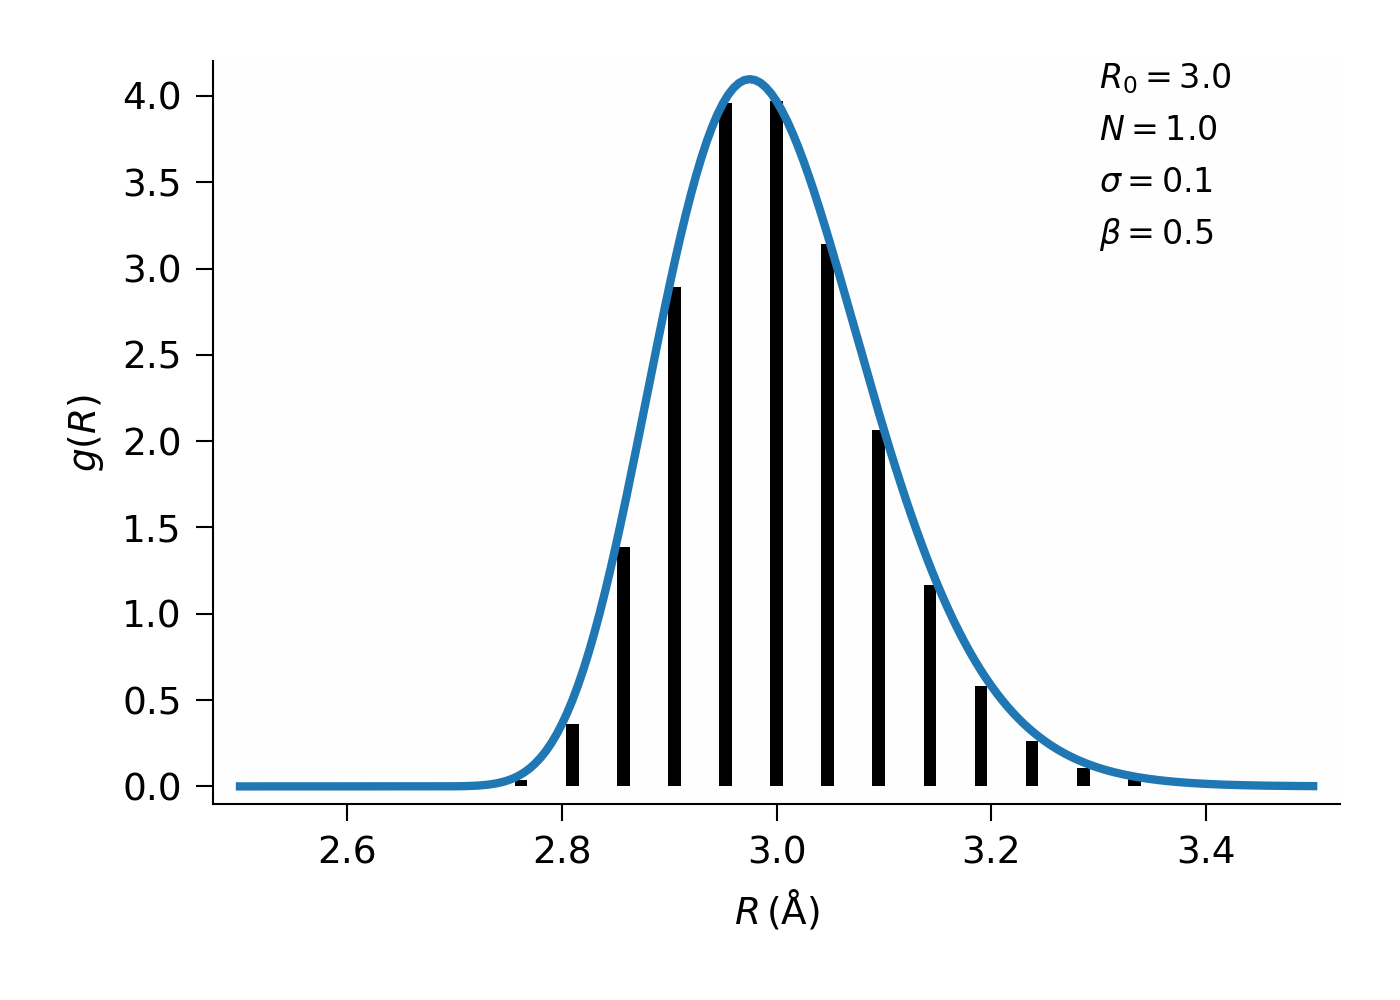
\includegraphics[width=60mm]{figs/errors/gnxas_histogram}
    \end{column}
  \end{columns}

  \end{cenpage}
\end{slide}


\section{Conclusions}
\begin{slide}{EXAFS Data Analysis with FEFF}


  \begin{cenpage}{126mm}

    Using {\feff} to model EXAFS mostly means paying attention to:

    \begin{itemize}
    \item   $N_{\rm idp}$ -- not very many
      Parameters can be varied for a limited $k$ and $R$ range.
    \item   Always look at the uncertainties in the Parameters, not just
      best-fit values.
    \item   Check (or require in the fit) that $\sigma^2 > 0$,  $N > 0$.
    \item   Think about how you might combine Parameters for different
      Paths, ideally making a physical model.
    \item  Try a third cumulant now and then -- it might be needed.
    \item   For very disordered systems, cumulants might not be enough.
    \end{itemize}

        \vmm     \hrule \vmm

  More information on X-rays and X-ray Absorption Spectroscopy:

  \begin{itemize}
  \item[] {\Blue{https://xafs.xrayabsorption.org/}}
  \item[] {\BlueEmph{Fundamentals of XAFS}} M. Newville, Reviews in  Mineralogy \& Geochemistry {\bf{78}}, 2014.
  \item[] {\BlueEmph{Introduction to XAFS}} G. Bunker, Cambridge Univ  Press,  2010.
  \item[] {\BlueEmph{XAFS for Everyone}} S. Calvin, CRC Press, 2013.
  \item[]  {\BlueEmph{Elements of Modern X-ray Physics}}  J.~Als-Nielsen
    \& D.~McMorrow,  John Wiley \& Sons. 2001

  \end{itemize}

\end{cenpage}


 \vfill
\end{slide}



\end{document}
